\chapter{Estado de la Cuestión} 
\section{Trabajos Relacionados}

Existen múltiples aplicaciones diseñadas para facilitar la búsqueda de eventos y establecimientos sociales. Por
ejemplo, aplicaciones como Yelp, Google y TripAdvisor permiten a los usuarios buscar restaurantes, bares, y eventos
según las reseñas y valoraciones de otros usuarios.

\begin{enumerate}
    \item \textbf{TripAdvisor:} Tripadvisor es la plataforma de orientación de viajes más grande del mundo. Ayuda a
          cientos de millones de personas cada mes en la planificación, reserva y realización de viajes. Los viajeros usan
          el sitio y la aplicación para descubrir alojamientos, actividades y restaurantes basados en las recomendaciones
          de otros viajeros.

    \item \textbf{Yelp:} Yelp conecta a las personas con excelentes negocios locales. Con información confiable
          sobre negocios locales, fotos y contenido de reseñas, Yelp proporciona una plataforma local integral para que
          los consumidores descubran, se conecten y realicen transacciones con negocios de todos los tamaños, facilitando
          la solicitud de presupuestos, la unión a listas de espera, la realización de reservas y la programación de citas
          o compras.

    \item \textbf{Google:} Google Maps permite a los turistas descubrir una amplia variedad de establecimientos de
          ocio, como restaurantes, bares, parques, museos y otros puntos de interés. La función de búsqueda integrada
          facilita encontrar lugares específicos o explorar categorías de interés en una zona determinada.

\end{enumerate}

A continuación, se muestran imágenes de las aplicaciones mencionadas:

\begin{figure}[H]
    \centering

    \begin{subfigure}{.3\textwidth}
        \centering
        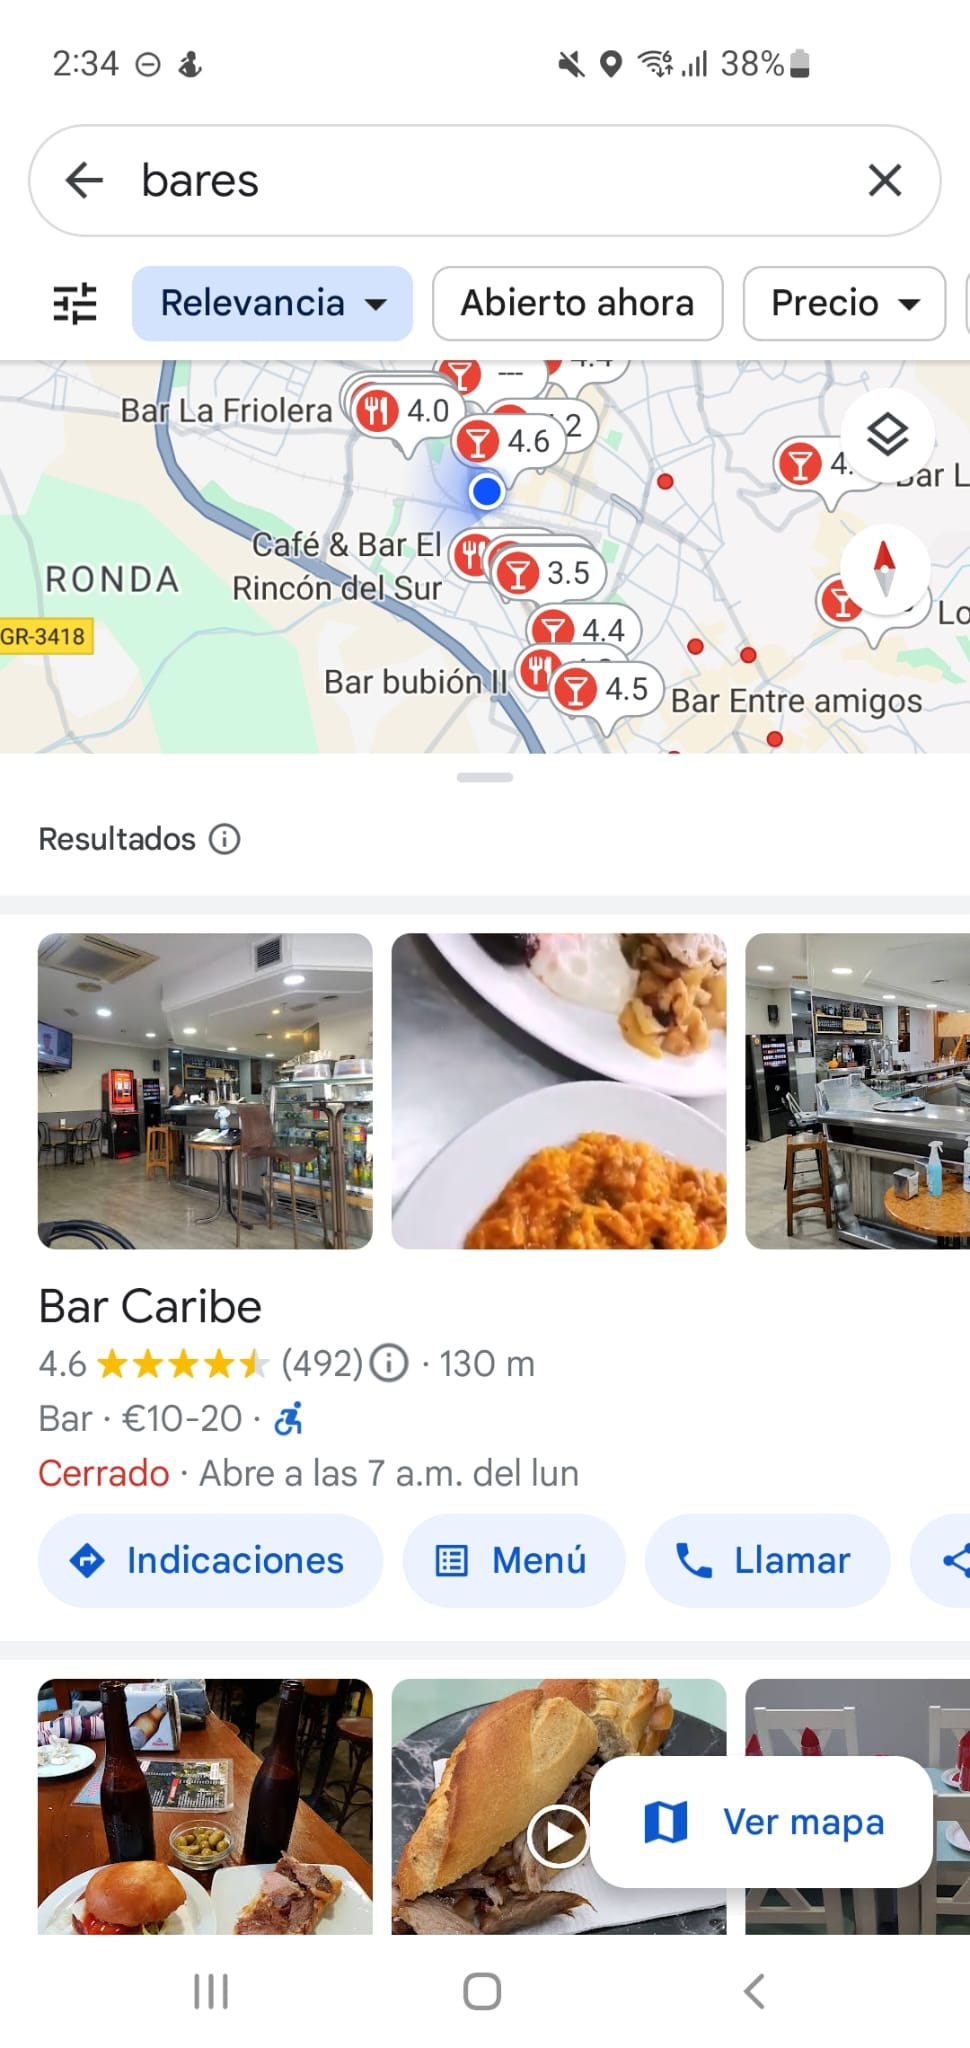
\includegraphics[width=\linewidth]{imagenes/GoogleMaps.jpeg}
        \caption{Google Maps}
        \label{fig:img1}
    \end{subfigure}%
    \hfill
    \begin{subfigure}{.3\textwidth}
        \centering
        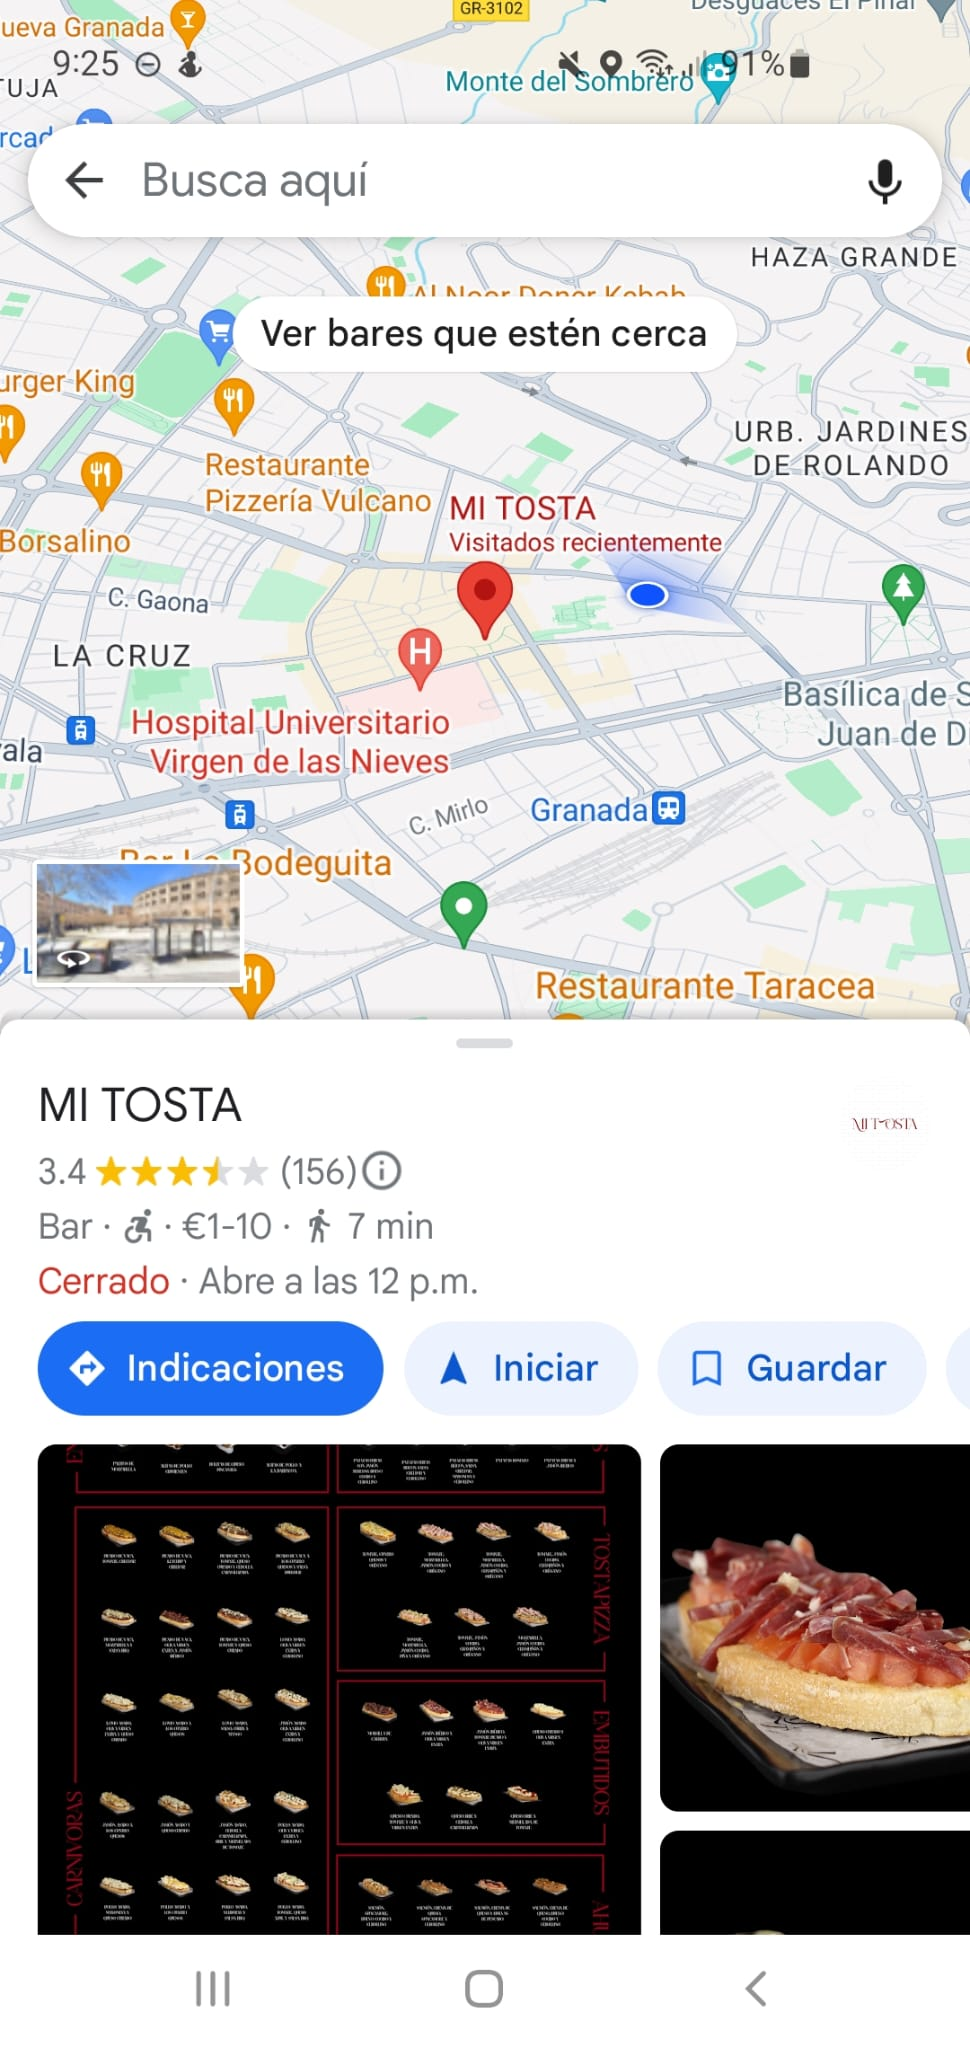
\includegraphics[width=\linewidth]{imagenes/Maps.jpeg}
        \caption{Google Maps}
        \label{fig:img2}
    \end{subfigure}%
    \hfill
    \begin{subfigure}{.3\textwidth}
        \centering
        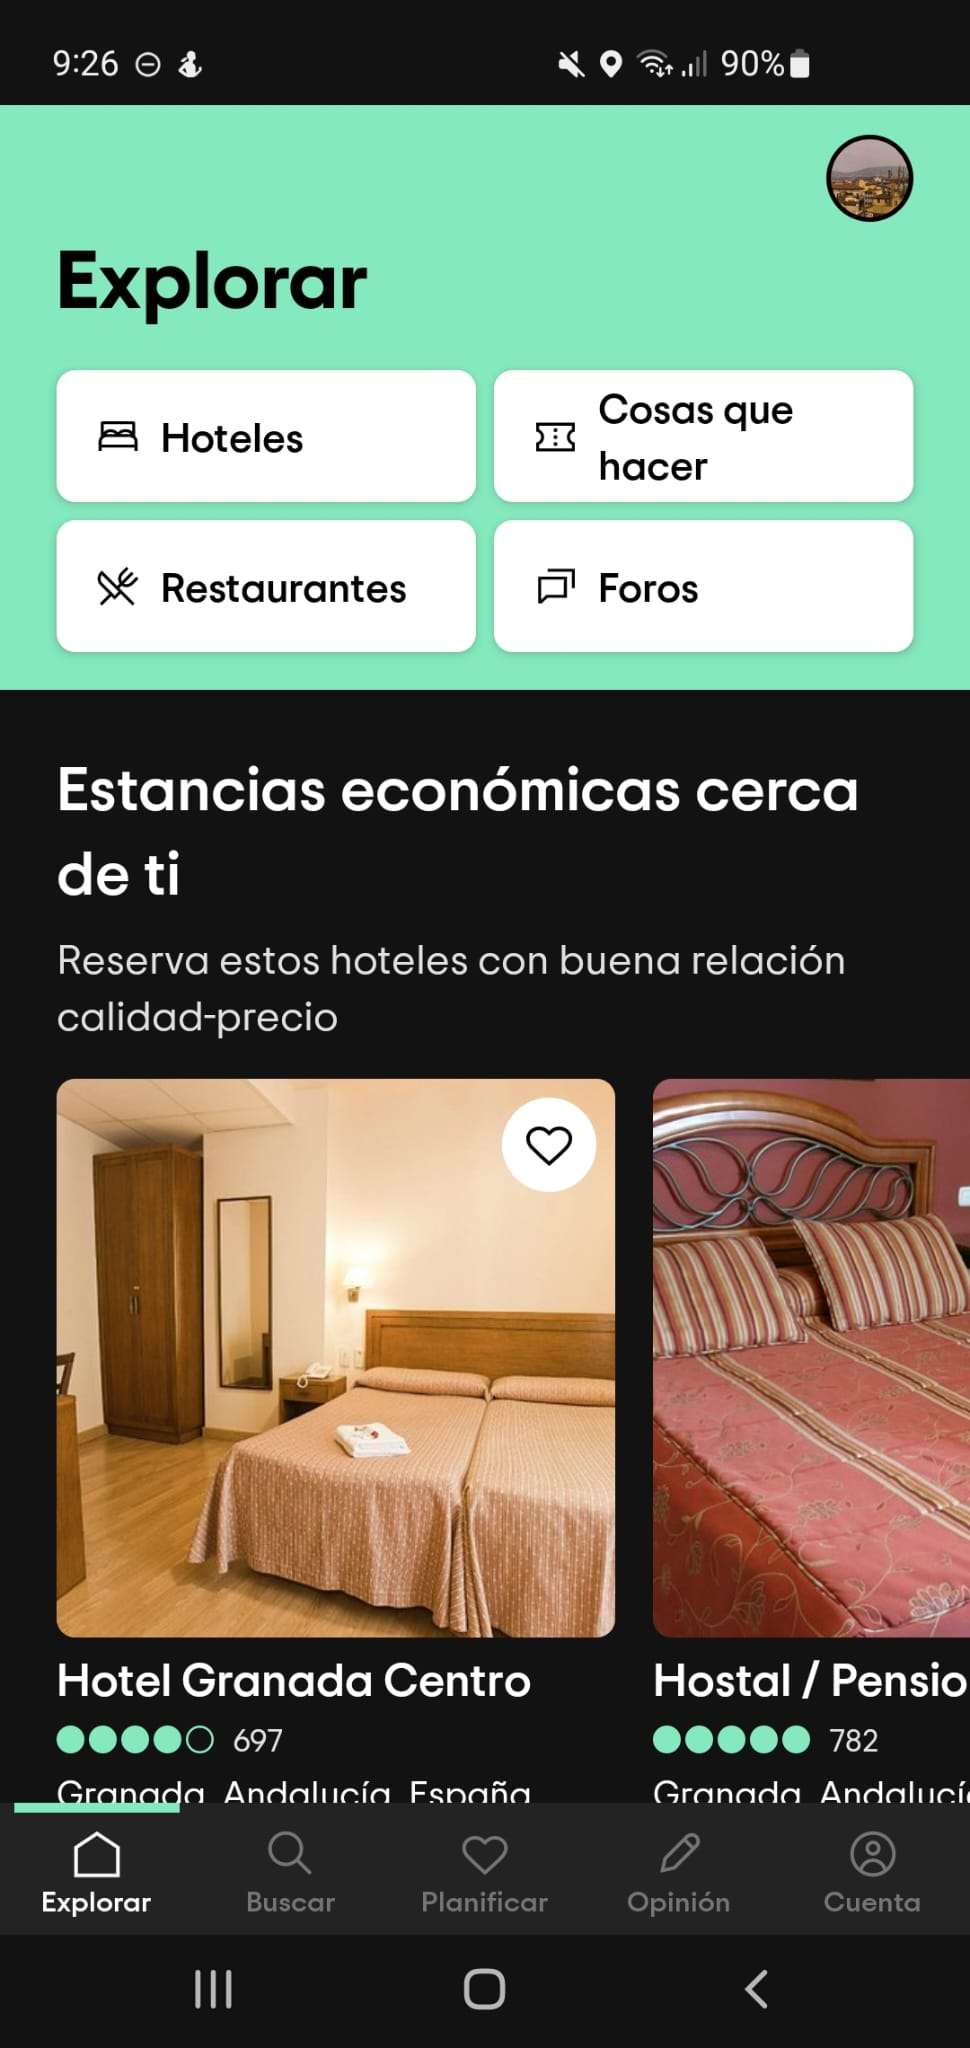
\includegraphics[width=\linewidth]{imagenes/TripAdvisor1.jpeg}
        \caption{TripAdvisor}
        \label{fig:img3}
    \end{subfigure}

    \vspace{1em}

    \begin{subfigure}{.3\textwidth}
        \centering
        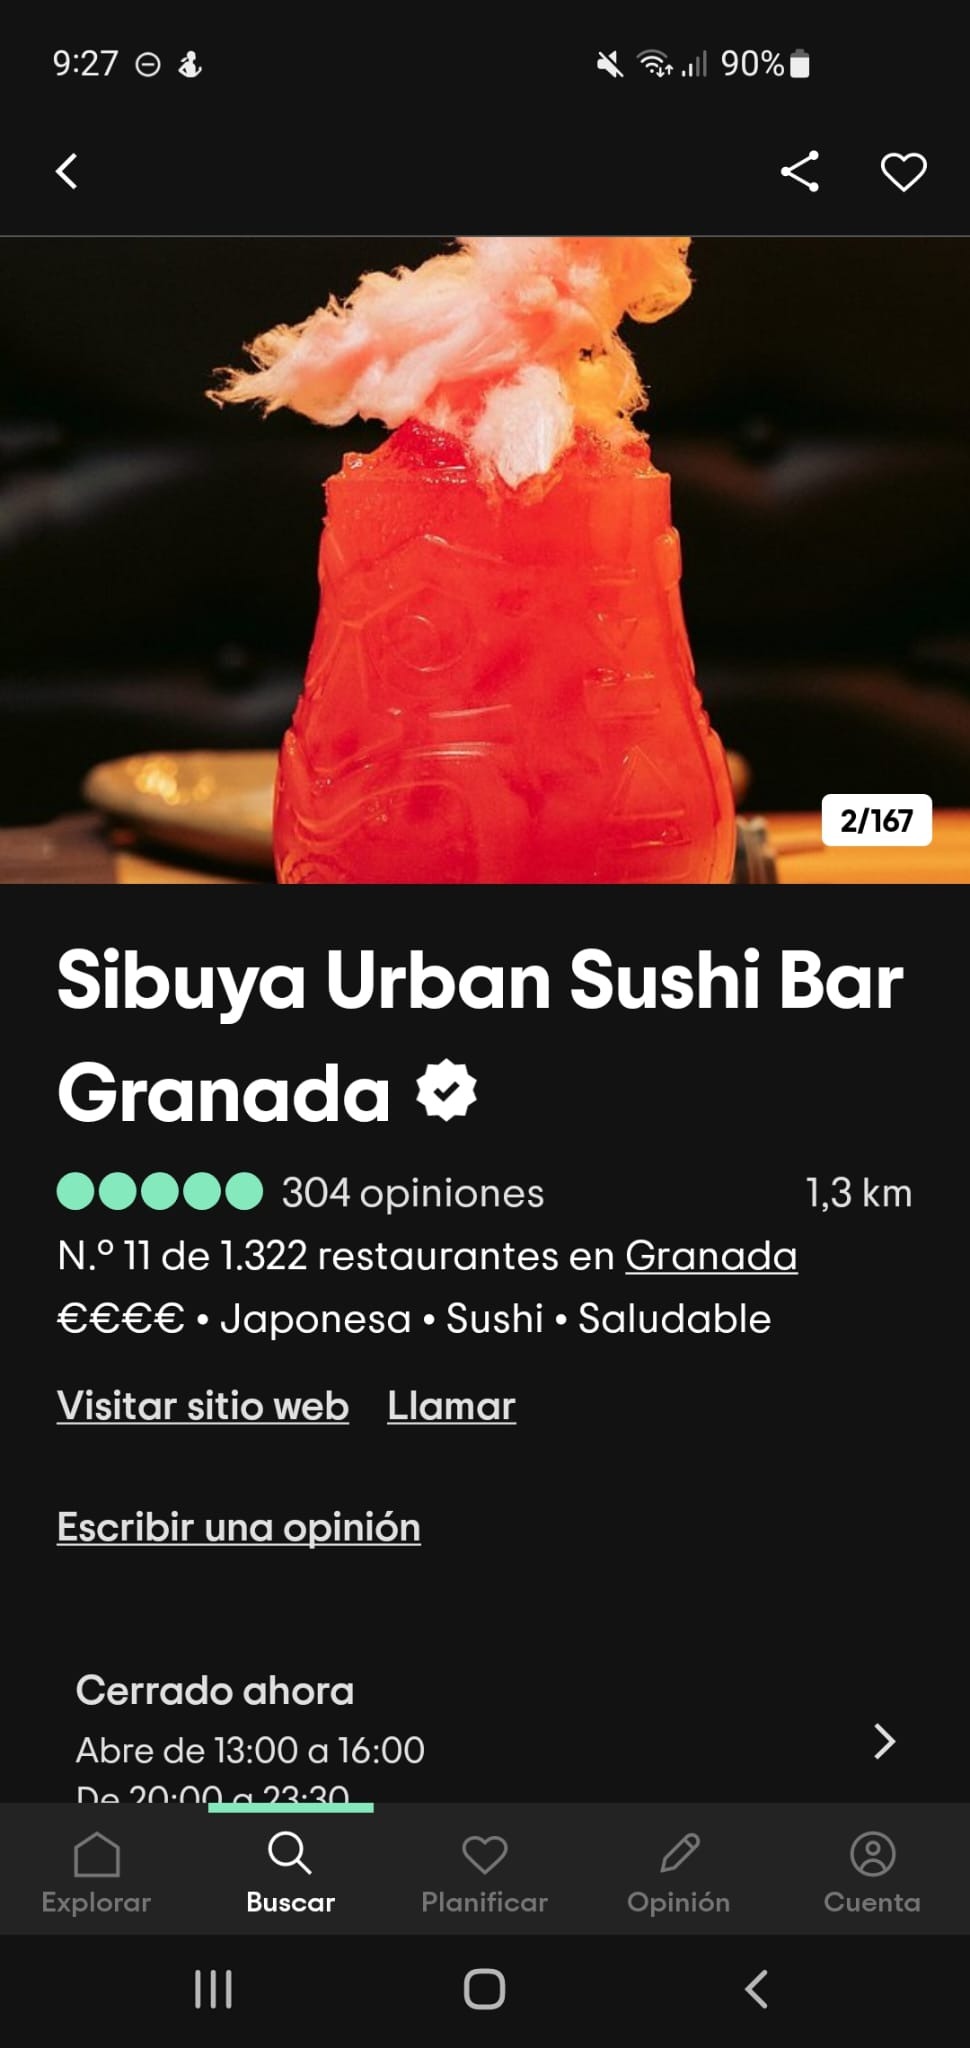
\includegraphics[width=\linewidth]{imagenes/TripAdvisor2.jpeg}
        \caption{TripAdvisor}
        \label{fig:img4}
    \end{subfigure}%
    \hfill
    \begin{subfigure}{.3\textwidth}
        \centering
        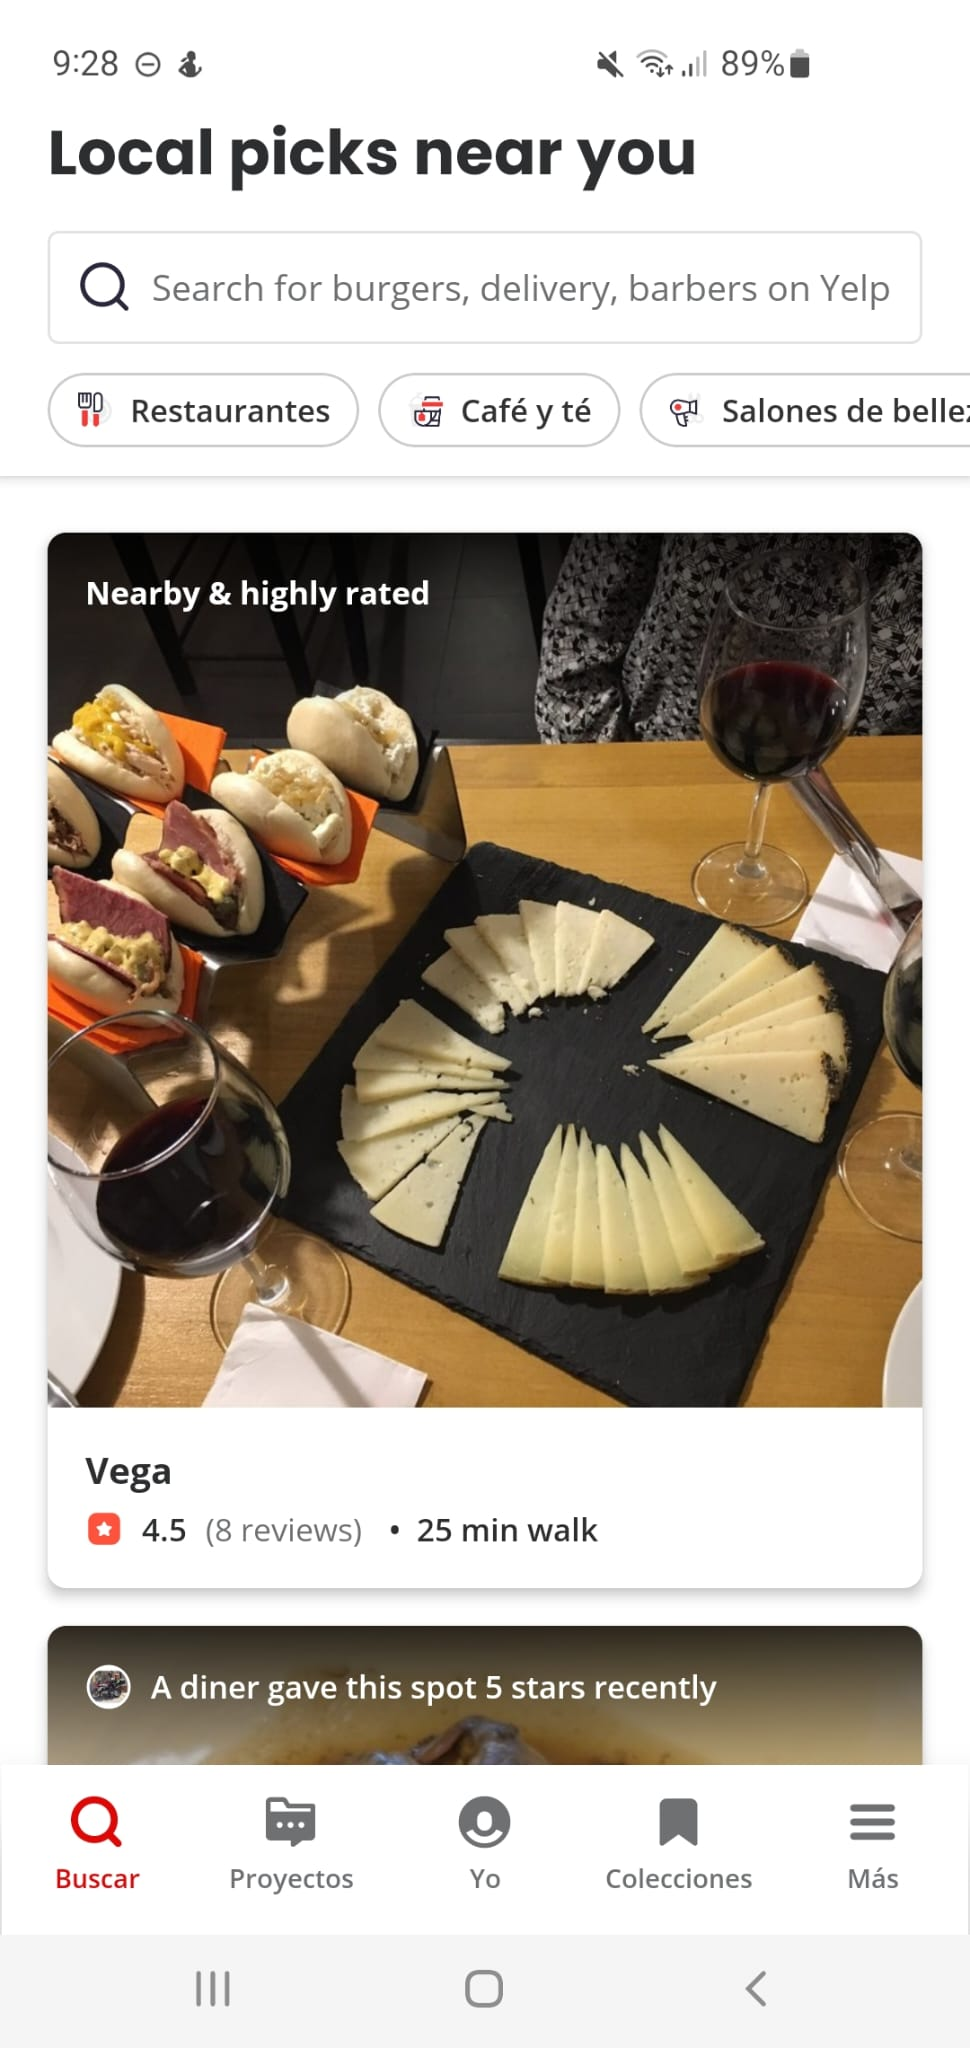
\includegraphics[width=\linewidth]{imagenes/Yelp1.jpeg}
        \caption{Yelp}
        \label{fig:img5}
    \end{subfigure}%
    \hfill
    \begin{subfigure}{.3\textwidth}
        \centering
        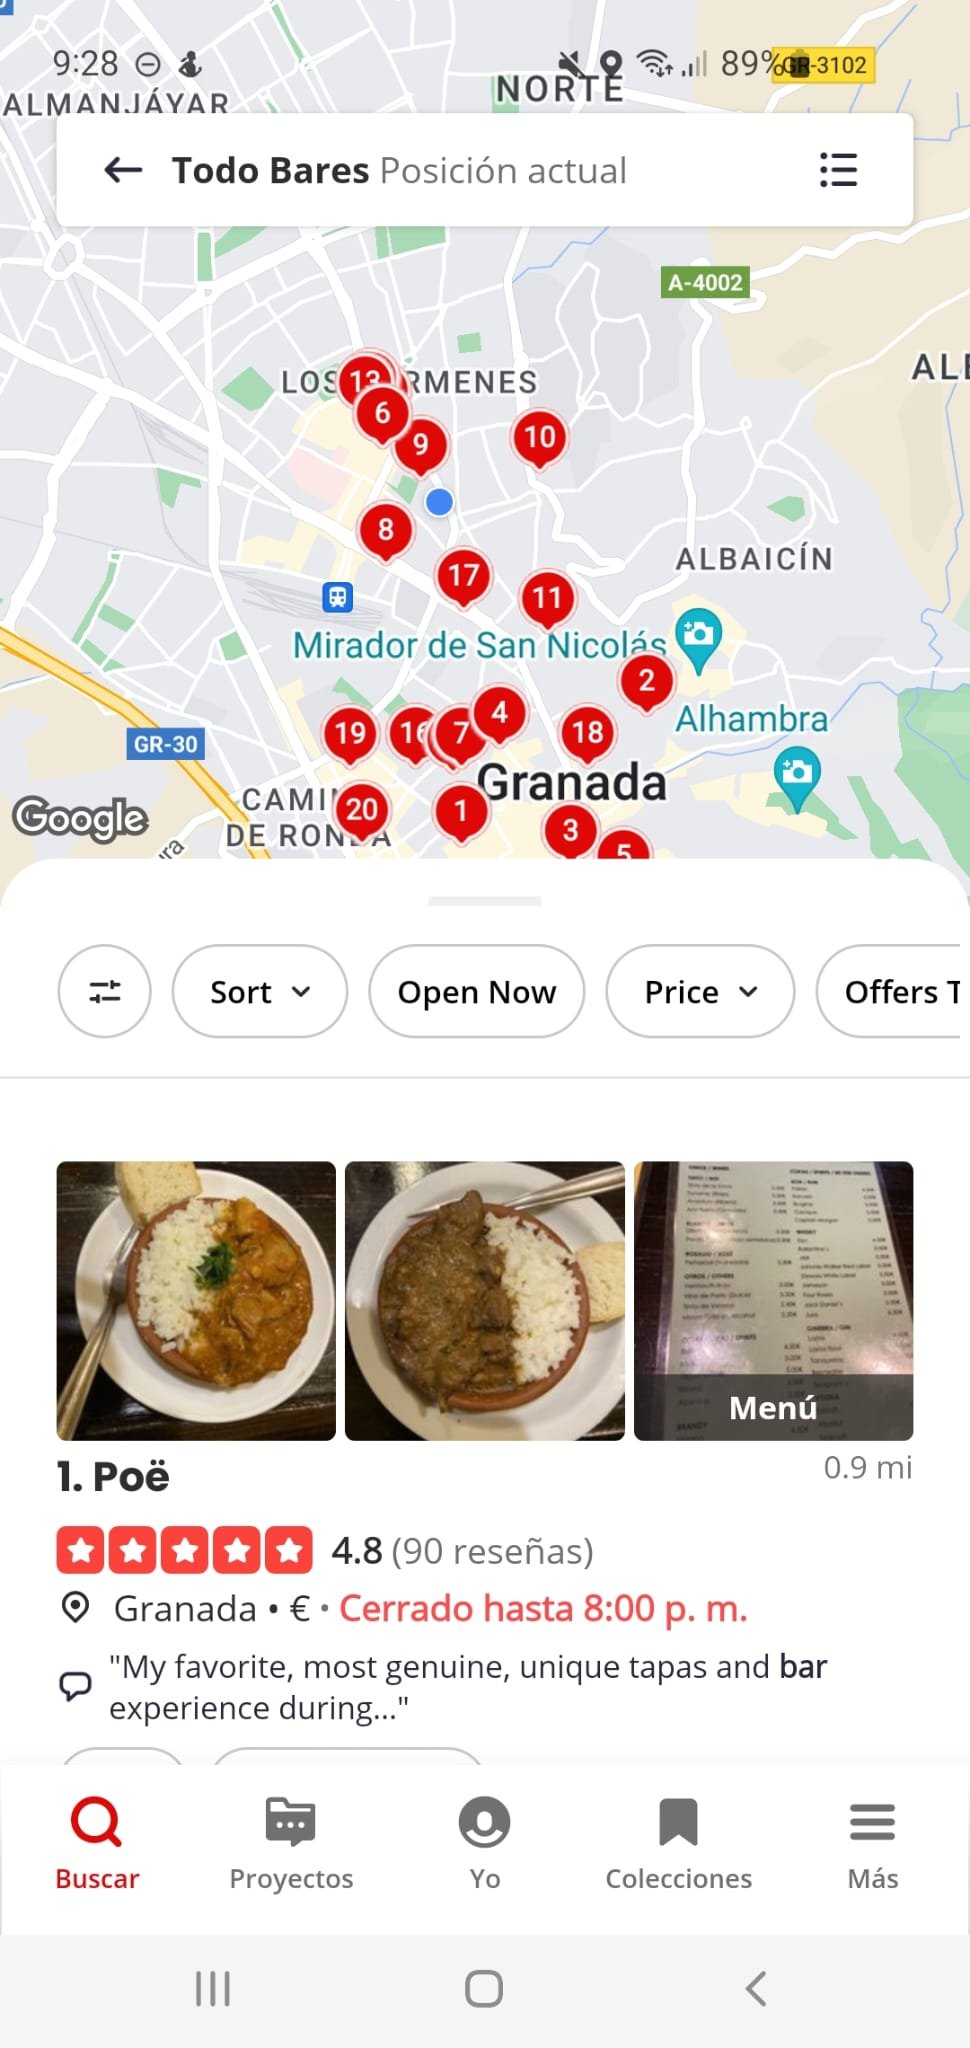
\includegraphics[width=\linewidth]{imagenes/Yelp2.jpeg}
        \caption{Yelp}
        \label{fig:img6}
    \end{subfigure}

    \caption{Comparación de aplicaciones orientadas al turismo}
    \label{fig:comparacion_apps}
\end{figure}

Además de estas opciones comerciales, existen otros proyectos académicos que siguen este mismo enfoque, por ejemplo:

\begin{enumerate}
    \item \textbf{Sebastián Alfredo Castro Rampersad}, \textit{Plataforma de Gestión y Venta de Entradas
              para locales de ocio nocturno}. Plataforma para la gestión y venta de entradas para locales de ocio nocturno, orientada a mejorar la experiencia tanto de los locales como de los consumidores. Permite a los locales publicar y gestionar entradas, mientras que los consumidores pueden adquirirlas de manera sencilla. La plataforma incluye una aplicación web administrativa para los locales, una aplicación móvil para el escaneo de entradas en el punto de acceso, y una aplicación móvil para la compra de entradas por parte de los consumidores \cite{Sebastian}.
    \item \textbf{Eduardo Campos Diago}, \textit{Aplicación Móvil para la Localización de Restaurantes}. Plataforma para la localización de restaurantes, diseñada para facilitar a los usuarios encontrar establecimientos basados en comidas específicas, aprovechando las capacidades de los dispositivos móviles con Android. Esta aplicación se orienta principalmente al turismo y ocio, permitiendo no solo encontrar restaurantes sino también evaluar platos y agregar nuevos restaurantes a la base de datos, actuando parcialmente como red social \cite{Campos}.
    \item \textbf{Raquel García del Val}, \textit{ Diseño de una Aplicación para Promover el Ocio Rural}. Aplicación diseñada para promover el turismo y el ocio rural al proporcionar una plataforma donde los usuarios pueden explorar y completar rutas de senderismo. Al finalizar las rutas, los usuarios reciben descuentos en restaurantes y comercios locales, incentivando así la exploración y el disfrute de las áreas rurales \cite{Garcia}.
\end{enumerate}

Las aplicaciones discutidas anteriormente ofrecen numerosas ventajas, destacándose por su robustez y la amplia base de usuarios que gestionan. Estas características aseguran una experiencia de usuario confiable y eficiente, lo cual es crucial para aplicaciones que manejan grandes volúmenes de datos y transacciones frecuentes.

Por otro lado, los trabajos mencionados ilustran claramente las ventajas de las soluciones tecnológicas actuales en la organización de actividades turísticas. Estas soluciones facilitan la planificación y ejecución de actividades, mejorando la accesibilidad a la información y optimizando la experiencia del turista.

Sin embargo, como ocurre con todas las soluciones tecnológicas, estas aplicaciones y trabajos también presentan ciertas limitaciones. Entre ellas se incluyen:

\begin{enumerate}

    \item \textbf{Información Fragmentada:} Los usuarios deben de consultar distintas plataformas y seguir a
          diversos establecimientos en sus redes sociales para estar al tanto de eventos u ofertas, lo que resulta en una
          experiencia fragmentada. Esta dispersión no es sólo ineficiente, sino que puede llevar a que los usuarios
          pierdan el interés y abandonen la búsqueda con consecuencia que pierdan una oportunidad importante de encontrar
          ese lugar que buscan.

    \item \textbf{Interacción Social Limitada:} Estas aplicaciones permiten leer reseñas y calificaciones en un
          establecimiento por parte de otros usuarios pero no permiten la creación de actividades entre amigos ni fomentan
          la organización y la interacción social.

    \item \textbf{Promoción y Gestión para Establecimientos:} La gestión de los perfiles y la promoción de eventos y
          ofertas en estas plataformas no es una prioridad. Estas aplicaciones tienden a centrarse más en la experiencia
          del usuario, ofreciendo calificaciones y reseñas de los establecimientos, pero no promueven activamente los
          lugares con los eventos y ofertas que pueden tener.

    \item \textbf{Enfoque Amplio y no Exclusivo al Ocio:} Estas aplicaciones abarcan un conjunto de funcionalidades
          no exclusivamente centradas en el ocio. Por ejemplo, TripAdvisor proporciona información sobre hoteles,
          atracciones turísticas y restaurantes, mientras que Google requiere búsquedas individuales de cada
          establecimiento hasta encontrar uno que se ajuste a las necesidades del usuario.

\end{enumerate}

\begin{landscape}
    \begin{table}
        \centering
        \caption{Comparación de características de aplicaciones para el turismo}
        \label{tab:comparison}
        \small
        \begin{tabularx}{\linewidth}{|X|X|X|X|X|X|X|}
            \hline
                                                   & \textbf{TripAdvisor} & \textbf{Yelp} & \textbf{Google Maps} & \textbf{Sebastián Castro} & \textbf{Eduardo Campos} & \textbf{Raquel García} \\ \hline
            \textbf{Búsqueda por Filtros}          & Sí                   & Sí            & Sí                   & Sí                        & Sí                      & Sí                     \\ \hline
            \textbf{Centralizado}                  & Sí                   & Sí            & Sí                   & Sí                        & Sí                      & Sí                     \\ \hline
            \textbf{Exclusivo}                     & No                   & No            & No                   & Sí                        & No                      & No                     \\ \hline
            \textbf{Organización Social}           & No                   & No            & No                   & No                        & No                      & No                     \\ \hline
            \textbf{Promoción de Establecimientos} & Sí                   & No            & No                   & Sí                        & No                      & Parcialmente           \\ \hline
        \end{tabularx}
    \end{table}
\end{landscape}

Todas estas limitaciones subrayan la necesidad de idear una nueva solución. En este contexto, surge \textit{HangOut}, una aplicación móvil diseñada para superar estos desafíos. La descripción detallada de la aplicación móvil, junto con sus funcionalidades y beneficios, será descrita en los siguientes capítulos.



